%
% ---------------------------------------------------------------
% Copyright (C) 2012-2018 Gang Li
% ---------------------------------------------------------------
%
% This work is the default powerdot-tuliplab style test file and may be
% distributed and/or modified under the conditions of the LaTeX Project Public
% License, either version 1.3 of this license or (at your option) any later
% version. The latest version of this license is in
% http://www.latex-project.org/lppl.txt and version 1.3 or later is part of all
% distributions of LaTeX version 2003/12/01 or later.
%
% This work has the LPPL maintenance status "maintained".
%
% This Current Maintainer of this work is Gang Li.
%
%

\documentclass[
 size=14pt,
 paper=smartboard,  %a4paper, smartboard, screen
 mode=present, 		%present, handout, print
 display=slides, 	% slidesnotes, notes, slides
 style=tuliplab,  	% TULIP Lab style
 pauseslide,
 fleqn,leqno]{powerdot}


%我自己增加的两端对其用
\usepackage{ragged2e}
\renewcommand{\raggedright}{\leftskip=0pt \rightskip=0pt plus 0cm}


\usepackage{cancel}
\usepackage{caption}
\usepackage{stackengine}
\usepackage{smartdiagram}
\usepackage{attrib}
\usepackage{amssymb}
\usepackage{amsmath} 
\usepackage{amsthm} 
\usepackage{mathtools}
\usepackage{rotating}
\usepackage{graphicx}
\usepackage{boxedminipage}
\usepackage{rotate}
\usepackage{calc}
\usepackage[absolute]{textpos}
\usepackage{psfrag,overpic}
\usepackage{fouriernc}
\usepackage{pstricks,pst-3d,pst-grad,pstricks-add,pst-text,pst-node,pst-tree}
\usepackage{moreverb,epsfig,subfigure}
\usepackage{color}
\usepackage{booktabs}
\usepackage{etex}
\usepackage{breqn}
\usepackage{multirow}
\usepackage{natbib}
\usepackage{bibentry}
\usepackage{gitinfo2}
\usepackage{siunitx}
\usepackage{nicefrac}
%\usepackage{geometry}
%\geometry{verbose,letterpaper}
\usepackage{media9}
\usepackage{animate}
%\usepackage{movie15}
\usepackage{auto-pst-pdf}

%\usepackage{breakurl}
\usepackage{fontawesome}
\usepackage{xcolor}
\usepackage{multicol}



\usepackage{verbatim}
\usepackage[utf8]{inputenc}
\usepackage{dtk-logos}
\usepackage{tikz}
\usepackage{adigraph}
%\usepackage{tkz-graph}
\usepackage{hyperref}
%\usepackage{ulem}
\usepackage{pgfplots}
\usepackage{verbatim}
\usepackage{fontawesome}


\usepackage{todonotes}
% \usepackage{pst-rel-points}
\usepackage{animate}
\usepackage{fontawesome}

\usepackage{listings}
\lstset{frameround=fttt,
frame=trBL,
stringstyle=\ttfamily,
backgroundcolor=\color{yellow!20},
basicstyle=\footnotesize\ttfamily}
\lstnewenvironment{code}{
\lstset{frame=single,escapeinside=`',
backgroundcolor=\color{yellow!20},
basicstyle=\footnotesize\ttfamily}
}{}


\usepackage{hyperref}
\hypersetup{ % TODO: PDF meta Data
  pdftitle={Kaggle sildes},
  pdfauthor={Wang Mingxi},
  pdfpagemode={FullScreen},
  pdfborder={0 0 0}
}


% \usepackage{auto-pst-pdf}
% package to show source code

\definecolor{LightGray}{rgb}{0.9,0.9,0.9}
\newlength{\pixel}\setlength\pixel{0.000714285714\slidewidth}
\setlength{\TPHorizModule}{\slidewidth}
\setlength{\TPVertModule}{\slideheight}
\newcommand\highlight[1]{\fbox{#1}}
\newcommand\icite[1]{{\footnotesize [#1]}}

\newcommand\twotonebox[2]{\fcolorbox{pdcolor2}{pdcolor2}
{#1\vphantom{#2}}\fcolorbox{pdcolor2}{white}{#2\vphantom{#1}}}
\newcommand\twotoneboxo[2]{\fcolorbox{pdcolor2}{pdcolor2}
{#1}\fcolorbox{pdcolor2}{white}{#2}}
\newcommand\vpspace[1]{\vphantom{\vspace{#1}}}
\newcommand\hpspace[1]{\hphantom{\hspace{#1}}}
\newcommand\COMMENT[1]{}

\newcommand\placepos[3]{\hbox to\z@{\kern#1
        \raisebox{-#2}[\z@][\z@]{#3}\hss}\ignorespaces}

\renewcommand{\baselinestretch}{1.2}


\newcommand{\draftnote}[3]{
	\todo[author=#2,color=#1!30,size=\footnotesize]{\textsf{#3}}	}
% TODO: add yourself here:
%
\newcommand{\gangli}[1]{\draftnote{blue}{GLi:}{#1}}
\newcommand{\shaoni}[1]{\draftnote{green}{sn:}{#1}}
\newcommand{\gliMarker}
	{\todo[author=GLi,size=\tiny,inline,color=blue!40]
	{Gang Li has worked up to here.}}
\newcommand{\snMarker}
	{\todo[author=Sn,size=\tiny,inline,color=green!40]
	{Shaoni has worked up to here.}}

%%%%%%%%%%%%%%%%%%%%%%%%%%%%%%%%%%%%%%%%%%%%%%%%%%%%%%%%%%%%%%%%%%%%%%%%
% title
% TODO: Customize to your Own Title, Name, Address
%
\title{The Final Report}
\author{
Wang Mingxi
\\
\\Jilin University
\\College of Computer Science and Technology
}
\date{\gitCommitterDate}
%\date{\today} %暂时手写改动

% Customize the setting of slides
\pdsetup{
% TODO: Customize the left footer, and right footer
rf=\href{http://www.tulip.org.au}{
Last Changed by: \textsc{\gitCommitterName}\ \gitVtagn-\gitAbbrevHash\ (\gitAuthorDate)
%Last Changed by: \textsc{Mingxi Wang}\ \gitVtagn-\gitAbbrevHash\ (\today)
},
cf={flip01-kaggle},
}


\begin{document}

\maketitle

%\begin{slide}{Overview}
%\tableofcontents[content=sections]
%\end{slide}


%%==========================================================================================
%%
\begin{slide}[toc=,bm=]{Overview}
\tableofcontents[content=currentsection,type=1]
\end{slide}
%%
%%==========================================================================================


\section{Research motivation and context}

%%==========================================================================================
%%
\begin{slide}{Project Objectives}

\begin{itemize}
\item Adversarial samples are generated on the MNIST dataset
\end{itemize}

\begin{center}
	\begin{figure}[htbp]
		
\includegraphics[scale=0.4]{./pic/1.eps}
	\end{figure}
\end{center}

\end{slide}
%%
%%==========================================================================================

%%==========================================================================================
%%
\begin{slide}{Project background}
\raggedright
In the real world, there are some unnatural data, they may be corroded existence, may be man-made.
It is interesting that these phenomena exist.
In the case of images, we can perturb some images so that the classifier fails, but it doesn't look different to the human eye.
This is called counterattack.
The purpose of this Kaggle project is to generate some of these "unnatural" images on the MNIST dataset to trick the classifier, while the human eye looks normal.
\end{slide}

\section{Research contents and methods}

%%
%%==========================================================================================
\begin{slide}{Import the MNIST dataset}
%当有多个Kaggle Subject而只想在目录出现一次时,在后面几次Kaggle Subject前加上[toc=,bm=]
	\raggedright
from subprocess import check_output\\
print(check_output(["ls", "../input"]).decode("utf8"))\\
df = pd.read_csv("../input/digit-recognizer/train.csv")\\
df.head()
\begin{center}
	\begin{figure}[htbp]
		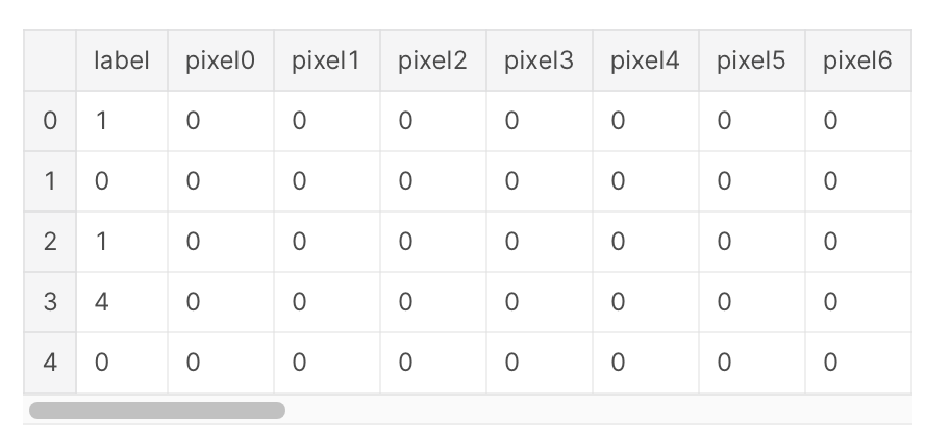
\includegraphics[scale=0.7]{./pic/2.eps}
	\end{figure}
\end{center}

\end{slide}

\begin{slide}{Split the training set and test set}
	\begin{itemize}
	\item 	The data set is divided into two parts: training set and testing set.\\
	\end{itemize}

y = df.label.values\\
X = df.drop("label",axis=1).values\\
X_train, X_test, y_train, y_test = train_test_split(X, y,test_size=0.4, random_state=0)\\

\end{slide}

\begin{slide}[toc=,bm=]{The initial preparation}
	\begin{itemize}
	\item Sort out the training set test set and train the classification model
	\end{itemize}
	self.images = X_test\\
        self.true_targets = y_test\\
        self.num_samples = X_test.shape[0]\\
        self.train(X_train, y_train)\\
        print("Model training finished.")\\
        self.test(X_test, y_test)\\
        print("Model testing finished. Initial accuracy score: " + str(self.initial_score))\\

\end{slide}

\begin{slide}{Get disturbance}
		gradient = gradient_method(target, pred_proba, self.weights)\\
inf_norm = np.max(gradient)\\
perturbation = epsilon/inf_norm * gradient\\

	\begin{itemize}
		\item The last line of code says, divide the gradient by the maximum element in the gradient, which is an operation that normalizes the gradient.
		Epsilon is an artificial input proportionality constant, which refers to how many times the gradient is magnified.
		The bigger it is, the bigger the gradient is going to be.
	\end{itemize}
	
	
\end{slide}

\begin{slide}{Attack function}
	
	def attack(self, attackmethod, epsilon):\\
        perturbed_images, highest_epsilon = self.perturb_images(epsilon, attackmethod)\\
        perturbed_preds = self.model.predict(perturbed_images)\\
        score = accuracy_score(self.true_targets, perturbed_preds)\\
        return perturbed_images, perturbed_preds, score, highest_epsilon\\
	\begin{itemize}
	\item 	The perturbed image is obtained, and the highest perturbation is obtained
	\end{itemize}
	
\end{slide}

\begin{slide}[toc=,bm=]{drawing I}
	sns.set()\\
	plt.figure(figsize=(10,5))\\
	plt.plot(attack.epsilons, attack.scores, 'g*')\\
	plt.ylabel('accuracy_score')\\
	plt.xlabel('epsilon')\\
	plt.title('Accuracy score breakdown - non-targeted attack')\\
	
\end{slide}

\begin{slide}[toc=,bm=]{drawing II}
		The greater the disturbance, the lower the accuracy of the model.The accuracy of the model declines fastest in the middle.But if the disturbance is too large, the human eye will not be able to distinguish the picture, and will lose the meaning of confrontation.
	\begin{center}
		\begin{figure}[htbp]
			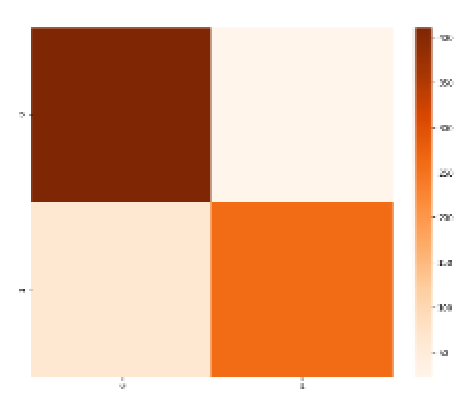
\includegraphics[scale=0.6]{./pic/3.eps}
		\end{figure}
	\end{center}
\end{slide}

\begin{slide}[toc=,bm=]{Experimental output display}
example_results = pd.DataFrame(data=attack.true_targets, columns=['y_true'])\\
example_results['y_fooled'] = example_preds\\
example_results['y_predicted'] = attack.preds\\
example_results['id'] = example_results.index.values\\
example_results.head()
		\begin{figure}[htbp]
			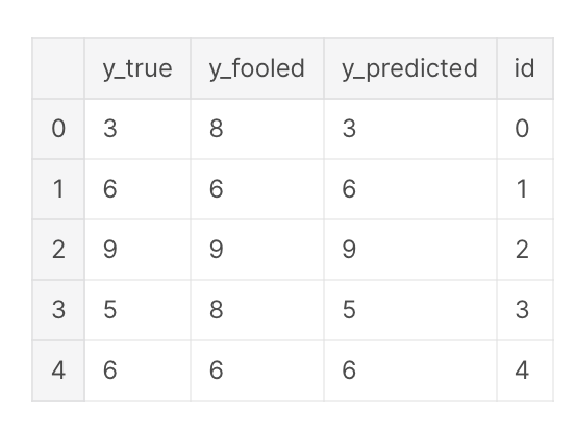
\includegraphics[scale=0.9]{./pic/4.eps}
		\end{figure}
	
\end{slide}

\section{Conclusion}


\begin{slide}{Data visualization and analysis I}
	\begin{itemize}
	\item 	The data distribution of fooled target is shown in the figure below
\end{itemize}

	\begin{figure}[htbp]
	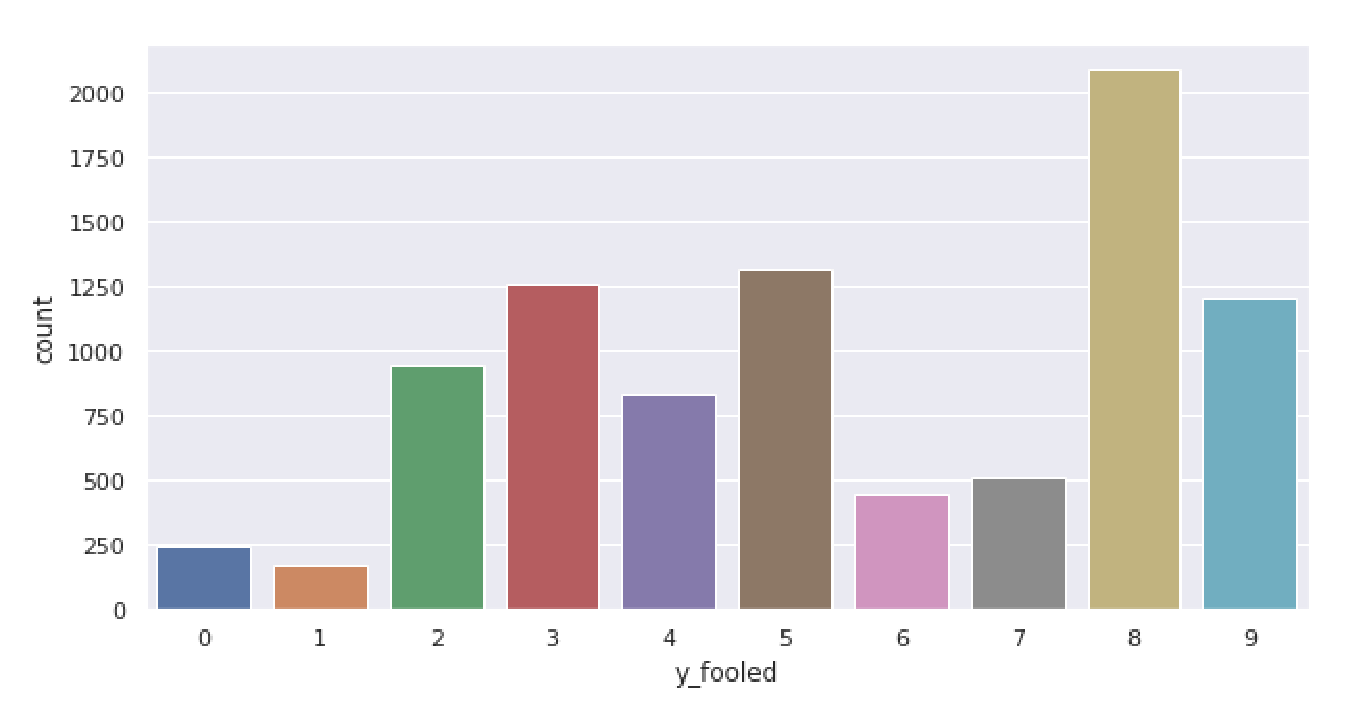
\includegraphics[scale=0.8]{./pic/5.eps}
	\end{figure}

\end{slide}
\begin{slide}{Data visualization and analysis II}
	
	We see that eight is often chosen as a target for deception, and this may have something to do with the internal characteristics of the number, which we don't know.\\
	Personally, it is because 8 is a centrally symmetric figure, so other numbers can imitate its features with the least amount of perturbation on average.\\
	Although 0 is also a centrally symmetric figure, : in that it is empty : the identification of the image as 0 requires additional perturbation, so the probability of Fooled Label being 0 is low.\\
	Because 2, 3, 5, and 9 share some similarities with 8 in their representation : in that they share a semicircular structure : the Fooled Target is only second to them in the probability that they were chosen.
	These phenomena imply the internal information of data characteristics, and the disturbance is the lateral representation of this information.
	
\end{slide}
%%
%%==========================================================================================

%%==========================================================================================
%%

%%
%%==========================================================================================



%%
%%==========================================================================================


%%==========================================================================================
% TODO: Contact Page
\begin{wideslide}[toc=,bm=]{Contact Information}
\centering
\vspace{\stretch{1}}
\twocolumn[
lcolwidth=0.35\linewidth,
rcolwidth=0.65\linewidth
]
{
% \centerline{
\includegraphics[scale=.2]{tulip-logo.eps}}
}
{
\vspace{\stretch{1}}
Wang Mingxi\\
College of Computer Science and Technology\\
Jilin University, China
\begin{description}
 \item[\textcolor{orange}{\faEnvelope}] \href{mailto:mxwang@tulip.academy}
 {\textsc{\footnotesize{mxwang@tulip.academy}}}

 \item[\textcolor{orange}{\faHome}] \href{http://www.tulip.org.au}
 {\textsc{\footnotesize{Team for Universal Learning and Intelligent Processing}}}
\end{description}
}
\vspace{\stretch{1}}
\end{wideslide}

\end{document}

\endinput
